% !TeX program = xelatex
% 编译：xelatex 06-冲激函数的性质.tex（VS Code 的 LaTeX Workshop 会读上一行，自动用 xelatex）
% 来源：2022 浙江大学《信号与系统》胡浩基老师，冲激函数 δ(t) 的性质（教材第 12 页式 1-38、1-40、1-42，第 24 页式 1-82；性质五见郑君里《信号与系统》）。
% 体例：五条性质逐条给出定义与证明；中间插入「两个函数相等」的勒贝格定义与可数集，作为性质三以后的证明工具；最后讲 δ(t) 的多种极限形式。
\documentclass[UTF8,a4paper,11pt]{ctexart}
\usepackage{amsmath,amssymb}
\usepackage{geometry}
\geometry{margin=2.4cm}
\usepackage{xcolor}
\usepackage{mdframed}
\usepackage{booktabs}
\usepackage{needspace}
\usepackage{array}
\usepackage{enumitem}
\usepackage{tikz}
\usetikzlibrary{arrows.meta,positioning,calc,patterns,decorations.pathreplacing}
\usepackage{float}
\usepackage{fancyhdr}
% 页眉页脚清空，只在右下角保留页号（含首页）
\fancypagestyle{plain}{%
  \fancyhf{}%
  \fancyfoot[R]{\thepage}%
  \renewcommand{\headrulewidth}{0pt}%
  \renewcommand{\footrulewidth}{0pt}}
\usepackage[hidelinks,unicode,bookmarksnumbered,bookmarksopen=true,bookmarksopenlevel=2,pdftitle={冲激函数的性质}]{hyperref}
\usepackage{bookmark}% XeTeX 下 hyperref 自带的大纲不生效，用 bookmark 宏包生成 PDF 书签（需编译两遍）

\setCJKmainfont{Songti SC}[BoldFont={Songti SC Bold}]
\setCJKsansfont{PingFang SC}

\newmdenv[backgroundcolor=blue!4,linecolor=blue!50!black,linewidth=1pt,innertopmargin=6pt,innerbottommargin=6pt]{rememberbox}
\newenvironment{remember}{\begin{rememberbox}\textbf{重点}\par\smallskip}{\end{rememberbox}}
\newmdenv[backgroundcolor=yellow!8,linecolor=orange!70!black,linewidth=1pt,innertopmargin=6pt,innerbottommargin=6pt]{notebox}
\newenvironment{note}{\begin{notebox}\textbf{说明}\par\smallskip}{\end{notebox}}

% ---------------------------------------------------------------- 画图用的小宏
% 坐标轴：\taxes[自变量名]{横轴起点}{横轴终点}{纵轴顶端}。原点标 0（放在左下，避开纵轴）。
\newcommand{\taxes}[4][t]{%
  \draw[->] (#2,0) -- (#3,0) node[right,font=\scriptsize] {$#1$};
  \draw[->] (0,-0.3) -- (0,#4);
  \node[anchor=north east,font=\tiny,gray!60!black,inner sep=1pt] at (0,-0.02) {$0$};}
% 不标原点 0 的坐标轴（原点附近另有刻度时用）
\newcommand{\taxesn}[4][t]{%
  \draw[->] (#2,0) -- (#3,0) node[right,font=\scriptsize] {$#1$};
  \draw[->] (0,-0.3) -- (0,#4);}
% 横轴刻度 \xt{位置}{标签}、纵轴刻度 \yt{位置}{标签}：刻度线 + 白底数字，不压曲线。
\newcommand{\xt}[2]{\draw (#1,0) -- (#1,-0.1) node[anchor=north,font=\tiny,gray!60!black,fill=white,inner sep=0.6pt] {$#2$};}
\newcommand{\yt}[2]{\draw (0,#1) -- (-0.1,#1) node[anchor=east,font=\tiny,gray!60!black,fill=white,inner sep=0.6pt] {$#2$};}
% 冲激箭头 \imp{位置}{画出的高度}{强度标签}
\newcommand{\imp}[3]{\draw[->,ultra thick,red!70!black] (#1,0) -- (#1,#2);
  \node[anchor=south,font=\tiny,red!70!black,inner sep=1pt] at (#1,#2) {#3};}
\tikzset{>=stealth,
  sig/.style={thick,blue!60!black},
  res/.style={thick,red!70!black}}

% ---------------------------------------------------------------- 标题层级
\definecolor{secblue}{RGB}{31,78,121}
\definecolor{exorange}{RGB}{190,90,10}
\definecolor{ptteal}{RGB}{0,110,110}
\ctexset{
  section={format=\raggedright\Large\bfseries\color{secblue},
           beforeskip=3.2ex plus 1ex minus .5ex, afterskip=1.4ex,
           aftertitle={\par\nobreak\vspace{-1.1ex}\noindent\textcolor{secblue}{\rule{\linewidth}{0.8pt}}\par\nobreak\vspace{0.6ex}}},
  subsection={format=\raggedright\large\bfseries\color{secblue},
              beforeskip=2.4ex plus .8ex minus .4ex, afterskip=1.0ex}
}
% 例题标题：\example{标题}{结论}{附注}，附注一般留空。左边橙色实心「例 n」，右边结论标签；同时进 PDF 大纲（第 3 级）。
\newcounter{ex}[section]
\newcommand{\example}[3]{%
  \refstepcounter{ex}\phantomsection
  \addcontentsline{toc}{subsubsection}{例 \theex\ #1（#2）}%
  \par\addvspace{1.6ex}\noindent
  {\setlength{\fboxsep}{3pt}%
   \colorbox{exorange}{\textcolor{white}{\textbf{例~\theex}}}\ %
   \textcolor{exorange}{\textbf{#1}}\ {\footnotesize\textcolor{gray!70!black}{#3}}%
   \hfill\colorbox{exorange!12}{\small\textcolor{exorange}{#2}}\par}%
  \nobreak\vskip0.6ex\relax\csname @afterheading\endcsname}
% 小标题（接着同一段往下写，不进大纲）：青色三角 + 粗体。
\newcommand{\point}[1]{\par\addvspace{1ex}\noindent\textcolor{ptteal}{$\blacktriangleright$\,\textbf{#1}}\ }

\title{冲激函数\ \texorpdfstring{$\delta(t)$}{δ(t)}\ 的性质\\\large 浙江大学 2022《信号与系统》（胡浩基）听课笔记（教材第 12、24 页）}
\author{}
\date{}

\begin{document}
\pagestyle{plain}
\maketitle

%==================================================================
\section{复习：冲激函数的定义}\label{sec:def}
\begin{remember}
$\delta_\Delta(t)$ 是从 $0$ 到 $\Delta$ 的方波，宽度 $\Delta$，高度 $\dfrac1\Delta$，面积为 $1$；
\[
\delta(t)=\lim_{\Delta\to0}\delta_\Delta(t).
\]
\end{remember}
下面的性质一、二直接从这个定义出发证明；性质三起要用到「两个函数相等」的新定义（第 \ref{sec:equal} 节）。

%==================================================================
\section{性质一：积分为 1}\label{sec:p1}
\begin{remember}
\[
\int_{-\infty}^{+\infty}\delta(t)\,\mathrm{d}t=1\qquad(\text{教材第 12 页式 1-38}).
\]
推广到任意上下限：
\[
\int_a^b\delta(t)\,\mathrm{d}t=
\begin{cases}
1, & a<0<b,\\
-1, & a>0>b,\\
0, & \text{其他（上下限同号）}.
\end{cases}
\]
\end{remember}

\point{证明。}对任意 $\Delta$，$\delta_\Delta(t)$ 的面积是 $\Delta\cdot\frac1\Delta=1$，即 $\int_{-\infty}^{+\infty}\delta_\Delta(t)\,\mathrm{d}t=1$。所以
\begin{align*}
\int_{-\infty}^{+\infty}\delta(t)\,\mathrm{d}t
&=\int_{-\infty}^{+\infty}\Big[\lim_{\Delta\to0}\delta_\Delta(t)\Big]\mathrm{d}t\\
&=\lim_{\Delta\to0}\int_{-\infty}^{+\infty}\delta_\Delta(t)\,\mathrm{d}t
&&\text{（$\delta(t)$ 的积分就\textbf{定义}为这个极限）}\\
&=\lim_{\Delta\to0}1=1.
\end{align*}

\point{推广的含义。}冲激只在 $t=0$ 一个点上「冲上去」。积分区间跨过 $0$（$a<0<b$）才积到它，结果为 $1$；反过来积（从大到小，$a>0>b$）按积分的定义变号，为 $-1$；区间不含 $0$（上下限都小于 $0$ 或都大于 $0$），积分为 $0$。

\begin{figure}[H]
\centering
\begin{tikzpicture}[x=1.4cm,y=1.1cm]
  \begin{scope}
    \taxes{-0.6}{1.8}{1.9}
    \fill[pattern=north east lines,pattern color=blue!50] (0,0) rectangle (0.7,1.4);
    \draw[sig] (0,0) -- (0,1.4) -- (0.7,1.4) -- (0.7,0);
    \xt{0.7}{\Delta}\yt{1.4}{\frac{1}{\Delta}}
    \node[anchor=west,font=\footnotesize] at (0.1,1.75) {$\delta_\Delta(t)$};
    \node[font=\scriptsize,fill=white,inner sep=1pt] at (1.25,0.7) {面积 $=1$};
  \end{scope}
  \begin{scope}[shift={(5.0,0)}]
    \taxes{-2.4}{3.2}{1.9}
    \imp{0}{1.3}{$(1)$}
    \foreach \p in {-2,-1,1,2,3}{\xt{\p}{\p}}
    \draw[decorate,decoration={brace,amplitude=3pt,mirror},green!50!black,thick] (-1,-0.45) -- (1.5,-0.45)
      node[midway,below=2pt,font=\scriptsize,green!40!black] {$a=-1,\ b=1.5$：积分 $=1$};
    \draw[decorate,decoration={brace,amplitude=3pt},gray,thick] (1,0.35) -- (2.6,0.35)
      node[midway,above=2pt,font=\scriptsize,gray!60!black] {$a=1,\ b=2.6$：积分 $=0$};
  \end{scope}
\end{tikzpicture}
\caption{左：每个 $\delta_\Delta(t)$ 的面积都是 $1$。右：积分区间跨过 $0$ 时积到冲激，结果为 $1$；区间不含 $0$ 时结果为 $0$。}
\end{figure}

%==================================================================
\section{性质二：筛选性}\label{sec:p2}
\begin{remember}
若 $x(t)$ 在 $t=0$ 处连续，则
\[
\int_{-\infty}^{+\infty}x(t)\,\delta(t)\,\mathrm{d}t=x(0)\qquad(\text{教材第 12 页式 1-40}).
\]
变形（冲激移到 $t_0$）：
\[
\int_{-\infty}^{+\infty}x(t)\,\delta(t-t_0)\,\mathrm{d}t=x(t_0).
\]
$x(t)$ 与冲激相乘再积分，只「筛」出冲激所在那一点的值。性质一是性质二在 $x(t)\equiv1$ 时的特例。
\end{remember}

\point{证明。}
\begin{align*}
\int_{-\infty}^{+\infty}x(t)\,\delta(t)\,\mathrm{d}t
&=\lim_{\Delta\to0}\int_{-\infty}^{+\infty}x(t)\,\delta_\Delta(t)\,\mathrm{d}t\\
&=\lim_{\Delta\to0}\int_0^\Delta x(t)\cdot\frac1\Delta\,\mathrm{d}t
&&\text{（$\delta_\Delta$ 只在 $[0,\Delta]$ 上非零，值为 $\tfrac1\Delta$）}\\
&=\lim_{\Delta\to0}\frac1\Delta\int_0^\Delta x(t)\,\mathrm{d}t\\
&=\lim_{\Delta\to0}\frac1\Delta\cdot x(\xi)\,\Delta,\quad 0\le\xi\le\Delta
&&\text{（积分中值定理）}\\
&=\lim_{\Delta\to0}x(\xi)=x(0)
&&\text{（$\xi$ 被夹在 $0$ 与 $\Delta$ 之间）}.
\end{align*}
\textbf{积分中值定理}：函数在一段区间上的积分，等于区间内某一点 $\xi$ 处的函数值乘区间长度。

\begin{figure}[H]
\centering
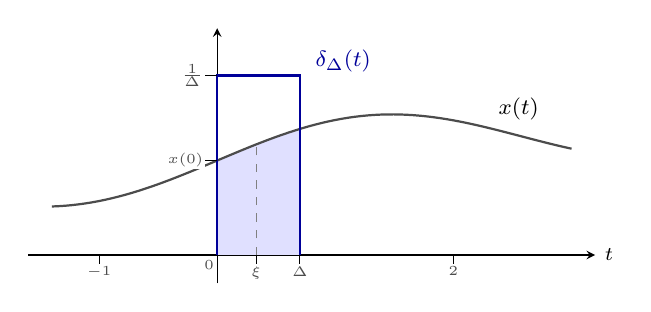
\begin{tikzpicture}[x=1.5cm,y=1.2cm]
  \taxes{-1.6}{3.2}{2.4}
  \fill[blue!12] (0,0) -- plot[domain=0:0.7,samples=20] (\x,{1+0.35*sin(70*\x)+0.1*\x}) -- (0.7,0) -- cycle;
  \draw[thick,gray!60!black,domain=-1.4:3,samples=80] plot (\x,{1+0.35*sin(70*\x)+0.1*\x});
  \draw[sig] (0,0) -- (0,1.9) -- (0.7,1.9) -- (0.7,0);
  \draw[dashed,gray] (0.33,0) -- (0.33,{1+0.35*sin(70*0.33)+0.033});
  \xt{0.33}{\xi}\xt{0.7}{\Delta}\xt{2}{2}\xt{-1}{-1}
  \yt{1}{x(0)}\yt{1.9}{\frac{1}{\Delta}}
  \node[anchor=west,font=\footnotesize] at (2.3,1.55) {$x(t)$};
  \node[anchor=west,font=\footnotesize,blue!60!black] at (0.75,2.05) {$\delta_\Delta(t)$};
\end{tikzpicture}
\caption{$x(t)\,\delta_\Delta(t)$ 只在 $[0,\Delta]$ 上非零。浅蓝色是 $\int_0^\Delta x(t)\,\mathrm{d}t=x(\xi)\Delta$，乘 $\frac1\Delta$ 后剩 $x(\xi)$；$\Delta\to0$ 时 $\xi\to0$，结果是 $x(0)$。}
\end{figure}

%==================================================================
\section{两个函数相等的定义}\label{sec:equal}
性质三 $x(t)\delta(t)=x(0)\delta(t)$ 的「$=$」两边都含冲激，不能逐点比较。要证明它，先要回答一个看似简单的问题：\textbf{两个函数 $f_1(t)$ 与 $f_2(t)$ 什么时候相等？}

\subsection{定义一：逐点相等}
\begin{remember}
\textbf{定义一}：若对任意 $t_0\in\mathbb{R}$，有 $f_1(t_0)=f_2(t_0)$，则 $f_1(t)=f_2(t)$。
\end{remember}
两条曲线必须\textbf{每一点都严丝合缝}地重合。这个定义\textbf{太严格}。

\begin{figure}[H]
\centering
\begin{tikzpicture}[x=1.3cm,y=1.1cm]
  \taxes{-0.5}{4.3}{2.4}
  \draw[thick,orange!80!black,domain=0:4,samples=60] plot (\x,{0.8+0.6*sin(60*\x)});
  \pgfmathsetmacro{\fv}{0.8+0.6*sin(120)}
  \draw[orange!80!black,fill=white,thick] (2,\fv) circle (2pt);
  \fill[red!70!black] (2,1.95) circle (2pt);
  \draw[dashed,gray] (2,0) -- (2,1.95);
  \xt{2}{t_0}\xt{1}{1}\xt{3}{3}\xt{4}{4}
  \yt{1}{1}\yt{2}{2}
  \node[anchor=west,font=\scriptsize,red!70!black] at (2.08,1.98) {$f_2(t_0)$};
  \node[anchor=west,font=\scriptsize,orange!80!black] at (2.1,{\fv-0.2}) {$f_1(t_0)$};
  \node[anchor=west,font=\footnotesize] at (3.3,0.55) {$f_1,f_2$ 其余点重合};
\end{tikzpicture}
\caption{两个函数只在 $t_0$ 一点不同。按定义一它们不相等；按下面的定义二、定义三它们相等。}
\end{figure}

\subsection{定义二：只在有限个点上不等}
如果只在一个点上不同也算相等，那么由等号的\textbf{传递性}，两个点、三个点……任意有限个点上不同也都必须算相等（中间插一个「只差一个点」的函数即可传递过去）。于是：

\begin{remember}
\textbf{定义二}：若 $f_1(t)$ 与 $f_2(t)$ 只在\textbf{有限个点}上不相等，在其他点上相等，则 $f_1(t)=f_2(t)$。
\end{remember}
这个定义可以用，但写法笨拙。

\subsection{定义三：勒贝格的定义}
\begin{remember}
\textbf{定义三}（勒贝格(Lebesgue)定义）：$f_1(t)=f_2(t)$ 是指对\textbf{任意}函数 $y(t)$，有
\[
\int_{-\infty}^{+\infty}y(t)\,f_1(t)\,\mathrm{d}t=\int_{-\infty}^{+\infty}y(t)\,f_2(t)\,\mathrm{d}t .
\]
\end{remember}
意思是：拿任意一个函数 $y(t)$ 去和它们分别相乘、再积分，结果总是一样，就认为这两个函数相等。

\point{定义三包含定义二。}若 $f_1$、$f_2$ 只在有限个点上不同，则 $y(t)f_1(t)$ 与 $y(t)f_2(t)$ 也只在这有限个点上不同；按黎曼积分的定义，改动有限个点上的值\textbf{不改变积分值}，所以两个积分相等。

\begin{note}
\begin{itemize}[nosep]
\item 「任意 $y(t)$」不包括 $\delta(t)$ 这类奇异函数：$y(t)$ 不能取冲激。
\item 「在有限个点上不等」指这些点上都是确定的有限值。若一个函数在某点有冲激、另一个没有，它们不相等。
\item 若某个 $y(t)$ 让积分不收敛（例如趋于 $+\infty$），则要求两边同时不收敛、且趋向相同。
\end{itemize}
\end{note}

\example{区间上不同的两个函数}{不相等}{}
\textbf{题目}：$f_1(t)$ 与 $f_2(t)$ 在 $[t_1,t_2]$ 以外处处相等，在 $[t_1,t_2]$ 上 $f_2(t)>f_1(t)$。按定义三，它们相等吗？

\textbf{解}：\textbf{不相等}。只需找一个反例 $y(t)$：取 $y(t)$ 在 $[t_1,t_2]$ 上为 $1$、其他地方为 $0$。则
\[
\int_{-\infty}^{+\infty}y(t)f_1(t)\,\mathrm{d}t=\int_{t_1}^{t_2}f_1(t)\,\mathrm{d}t,\qquad
\int_{-\infty}^{+\infty}y(t)f_2(t)\,\mathrm{d}t=\int_{t_1}^{t_2}f_2(t)\,\mathrm{d}t .
\]
由于 $t_1\le t\le t_2$ 时 $f_2(t)>f_1(t)$，所以后者严格大于前者，两个积分不等。哪怕这一段区间很短，两个函数也不相等。

\begin{figure}[H]
\centering
\begin{tikzpicture}[x=1.1cm,y=1.1cm]
  \begin{scope}
    \taxes{-0.5}{4.6}{2.3}
    \draw[thick,orange!80!black,domain=0:4.2,samples=60] plot (\x,{0.7+0.25*\x});
    \draw[res] (1.5,{0.7+0.375}) .. controls (1.8,1.9) and (2.4,1.9) .. (2.7,{0.7+0.675});
    \draw[dashed,gray] (1.5,0) -- (1.5,1.075);
    \draw[dashed,gray] (2.7,0) -- (2.7,1.375);
    \xt{1.5}{t_1}\xt{2.7}{t_2}\xt{4}{4}
    \yt{1}{1}\yt{2}{2}
    \node[anchor=west,font=\scriptsize,orange!80!black] at (3.4,1.75) {$f_1(t)$};
    \node[anchor=south,font=\scriptsize,red!70!black] at (2.1,1.8) {$f_2(t)$};
  \end{scope}
  \begin{scope}[shift={(6.5,0)}]
    \taxes{-0.5}{4.6}{2.3}
    \draw[sig] (0,0) -- (1.5,0) -- (1.5,1) -- (2.7,1) -- (2.7,0) -- (4.2,0);
    \xt{1.5}{t_1}\xt{2.7}{t_2}\xt{4}{4}
    \yt{1}{1}
    \node[anchor=west,font=\footnotesize] at (0.15,2.1) {反例 $y(t)$};
  \end{scope}
\end{tikzpicture}
\caption{左：$f_2$ 只在 $[t_1,t_2]$ 上高于 $f_1$。右：取 $y(t)$ 为 $[t_1,t_2]$ 上的方波，两个积分不等，所以 $f_1\ne f_2$。}
\end{figure}

\example{单位阶跃 u(t) 在 0 点的取值}{可以任取}{}
\textbf{题目}：$u(t)=\begin{cases}1,&t>0\\0,&t<0\end{cases}$，$u(0)$ 等于多少？

\textbf{解}：可以是任意值。设
\[
u_1(t)=\begin{cases}1,&t\ge0\\0,&t<0\end{cases},\qquad
u_2(t)=\begin{cases}1,&t>0\\0,&t\le0\end{cases}.
\]
两者只在 $t=0$ 一点不同，任何 $y(t)$ 与它们相乘后积分都一样。由定义三，$u_1(t)=u_2(t)$，是同一个函数。

\begin{figure}[H]
\centering
\begin{tikzpicture}[x=1.0cm,y=1.0cm]
  \begin{scope}
    \taxes{-2}{2.6}{1.8}
    \draw[sig] (-1.8,0) -- (-0.07,0);
    \draw[sig] (0,1) -- (2.2,1);
    \fill[blue!60!black] (0,1) circle (2pt);
    \draw[blue!60!black,fill=white,thick] (0,0) circle (2pt);
    \xt{-1}{-1}\xt{1}{1}\xt{2}{2}\yt{1}{1}
    \node[anchor=west,font=\footnotesize] at (0.15,1.6) {$u_1(t)$：$u_1(0)=1$};
  \end{scope}
  \begin{scope}[shift={(6,0)}]
    \taxes{-2}{2.6}{1.8}
    \draw[sig] (-1.8,0) -- (0,0);
    \draw[sig] (0.07,1) -- (2.2,1);
    \fill[blue!60!black] (0,0) circle (2pt);
    \draw[blue!60!black,fill=white,thick] (0,1) circle (2pt);
    \xt{-1}{-1}\xt{1}{1}\xt{2}{2}\yt{1}{1}
    \node[anchor=west,font=\footnotesize] at (0.15,1.6) {$u_2(t)$：$u_2(0)=0$};
  \end{scope}
\end{tikzpicture}
\caption{实心点是该点的取值，空心点表示不取。两者只差 $t=0$ 一个点，按定义三是同一个函数。}
\end{figure}

\example{系统 y(t)=t·x(t) 是否可逆}{可逆}{}
\textbf{题目}：系统 $y(t)=t\,x(t)$ 可逆吗？

\textbf{解}：$t\ne0$ 时 $x(t)=y(t)/t$，可以由输出恢复输入；只有 $t=0$ 一个点恢复不出来。按定义三，只差一个点的两个函数是同一个函数，所以可以认为这个系统可逆。

\begin{note}
平时做题不必走极端：例如问 $u(3)$ 等于多少，答 $1$ 即可。「在个别点上取值可以任意」只用于理解两个函数为什么相等，不要拿来否定常规的结论。
\end{note}

\subsection{勒贝格积分：横着数钱}
\point{黎曼积分(Riemann integral)。}高等数学里学的积分：把横轴切成一小段一小段，每段竖着取一个小矩形再相加。勒贝格的比喻是\textbf{「竖着数钱」}。

\point{勒贝格积分(Lebesgue integral)。}把\textbf{纵轴}切成一层一层，每一层横着取出函数值落在这一层的那些 $t$，再相加，即\textbf{「横着数钱」}。

\begin{figure}[H]
\centering
\begin{tikzpicture}[x=1.0cm,y=1.1cm]
  \begin{scope}
    \taxes{-0.4}{4.5}{2.3}
    \foreach \a in {0,0.5,...,3.5}{%
      \pgfmathsetmacro{\h}{0.3+1.5*exp(-((\a+0.25)-2)^2/1.2)}
      \draw[blue!60!black,fill=blue!12] (\a,0) rectangle ({\a+0.5},\h);}
    \draw[thick,gray!60!black,domain=0:4,samples=60] plot (\x,{0.3+1.5*exp(-(\x-2)^2/1.2)});
    \foreach \p in {1,2,3,4}{\xt{\p}{\p}}\yt{1}{1}
    \node[anchor=west,font=\footnotesize] at (0.15,2.15) {黎曼：竖着切};
  \end{scope}
  \begin{scope}[shift={(6.2,0)}]
    \taxes{-0.4}{4.5}{2.3}
    \fill[orange!20] (0,0) rectangle (4,0.3);
    \draw[orange!70!black] (0,0) rectangle (4,0.3);
    \foreach \L in {0.6,0.9,1.2,1.5,1.8}{%
      \pgfmathsetmacro{\w}{sqrt(-1.2*ln((\L-0.3)/1.5))}
      \draw[orange!70!black,fill=orange!20] ({2-\w},{\L-0.3}) rectangle ({2+\w},\L);}
    \draw[thick,gray!60!black,domain=0:4,samples=60] plot (\x,{0.3+1.5*exp(-(\x-2)^2/1.2)});
    \foreach \p in {1,2,3,4}{\xt{\p}{\p}}\yt{1}{1}
    \node[anchor=west,font=\footnotesize] at (0.15,2.15) {勒贝格：横着切};
  \end{scope}
\end{tikzpicture}
\caption{同一个函数的两种近似求面积方法。左：按 $t$ 切成竖条；右：按函数值切成横条，每条的长度是「函数值不低于这一层的 $t$ 的范围」。}
\end{figure}

\begin{remember}
\begin{itemize}[nosep]
\item 凡是黎曼可积的函数，勒贝格积分也能积，而且结果一样。
\item 有些函数黎曼积分积不出来，勒贝格积分能积。经典例子是\textbf{狄利克雷函数}(Dirichlet function)：
\[
D(t)=\begin{cases}1,&t\text{ 为有理数}\\0,&t\text{ 为无理数}\end{cases},\qquad
\int_0^1D(t)\,\mathrm{d}t=0\ (\text{勒贝格积分}).
\]
任意小的区间里都既有有理数又有无理数，竖着切怎么切都积不出来。
\item 用勒贝格积分理解定义三，定义二中的「有限个点」可以放宽为\textbf{可数个点}（第 \ref{sec:count} 节）：两个函数在可数个点上不等、其他点相等，仍然相等。例如两个函数在所有有理数点上都不等、在所有无理数点上相等，它们仍然相等。
\end{itemize}
\end{remember}

%==================================================================
\section{可数集与不可数集}\label{sec:count}
无限集合分为两类：\textbf{可数无限集}（简称可数集(countable set)）和\textbf{不可数集}(uncountable set)。这个区分由康托(Cantor)给出，是实变函数的基础。

\subsection{两个无限集「一样多」}
\begin{remember}
若存在一个由无限集 $A$ 到无限集 $B$ 的\textbf{一一映射}(bijection)，就称 $A$ 与 $B$ \textbf{一样多}，也叫\textbf{等势}或\textbf{基数相同}。

一一映射：$A$ 中每个元素唯一对应 $B$ 中一个元素，$B$ 中每个元素也唯一对应 $A$ 中一个元素，\textbf{没有重复，也没有遗漏}。
\end{remember}

\example{自然数与偶数}{一样多}{}
对应 $n\leftrightarrow 2n$：
\begin{center}
\begin{tabular}{@{}l|cccccc@{}}
\toprule
自然数 & $1$ & $2$ & $3$ & $4$ & $5$ & $\cdots$\\
偶数 & $2$ & $4$ & $6$ & $8$ & $10$ & $\cdots$\\
\bottomrule
\end{tabular}
\end{center}
没有重复也没有遗漏，所以自然数与偶数一样多。同理，自然数与奇数也一样多。

\example{自然数与整数}{一样多}{}
按 $0,1,-1,2,-2,3,-3,\dots$ 的顺序编号：
\begin{center}
\begin{tabular}{@{}l|cccccccccc@{}}
\toprule
自然数 & $1$ & $2$ & $3$ & $4$ & $5$ & $6$ & $7$ & $8$ & $9$ & $\cdots$\\
整数 & $0$ & $1$ & $-1$ & $2$ & $-2$ & $3$ & $-3$ & $4$ & $-4$ & $\cdots$\\
\bottomrule
\end{tabular}
\end{center}
每个整数都排到了一个位置，所以一样多。

\example{自然数与有理数}{一样多}{}
有理数都能写成 $\frac mn$（$m,n$ 为整数）。先把所有正有理数排成一张表：第 $n$ 行是分母为 $n$ 的数（重复的如 $\frac22$ 也先写上占位）。再按康托的\textbf{折线排序}走一遍：

\begin{figure}[H]
\centering
\begin{tikzpicture}[x=1.15cm,y=0.9cm]
  \foreach \n in {1,...,4}{%
    \node[font=\footnotesize,anchor=east] at (0.3,-\n) {$n=\n$};
    \foreach \m in {1,...,5}{%
      \node[font=\small] (q\m\n) at (\m,-\n) {$\frac{\m}{\n}$};}}
  \foreach \m/\n in {2/2,4/2,3/3,2/4,4/4}{\node[font=\small,gray!50,fill=white,inner sep=1pt] at (\m,-\n) {$\frac{\m}{\n}$};}
  \draw[->,thick,red!70!black,shorten <=6pt,shorten >=6pt]
    (q11) -- (q21);
  \draw[->,thick,red!70!black,shorten <=6pt,shorten >=6pt] (q21) -- (q12);
  \draw[->,thick,red!70!black,shorten <=6pt,shorten >=6pt] (q12) -- (q13);
  \draw[->,thick,red!70!black,shorten <=6pt,shorten >=6pt] (q13) -- (q22);
  \draw[->,thick,red!70!black,shorten <=6pt,shorten >=6pt] (q22) -- (q31);
  \draw[->,thick,red!70!black,shorten <=6pt,shorten >=6pt] (q31) -- (q41);
  \draw[->,thick,red!70!black,shorten <=6pt,shorten >=6pt] (q41) -- (q32);
  \draw[->,thick,red!70!black,shorten <=6pt,shorten >=6pt] (q32) -- (q23);
  \draw[->,thick,red!70!black,shorten <=6pt,shorten >=6pt] (q23) -- (q14);
  \draw[->,thick,red!70!black,dashed,shorten <=6pt] (q14) -- ++(0,-0.9);
  \node[font=\footnotesize] at (5.9,-1) {$\cdots$};
  \node[font=\footnotesize] at (3,-4.8) {$\vdots$};
\end{tikzpicture}
\caption{折线排序：$\frac11\to\frac21\to\frac12\to\frac13\to\frac22\to\frac31\to\frac41\to\frac32\to\frac23\to\frac14\to\cdots$。灰色的 $\frac22,\frac42,\frac33,\frac24,\frac44$ 与前面重复，走到时跳过。}
\end{figure}

编号时先放 $0$，之后每走到一个新的正有理数，就紧跟着写上它的相反数：
\begin{center}
\begin{tabular}{@{}l|ccccccccccc@{}}
\toprule
自然数 & $1$ & $2$ & $3$ & $4$ & $5$ & $6$ & $7$ & $8$ & $9$ & $10$ & $\cdots$\\
有理数 & $0$ & $1$ & $-1$ & $2$ & $-2$ & $\frac12$ & $-\frac12$ & $\frac13$ & $-\frac13$ & $3$ & $\cdots$\\
\bottomrule
\end{tabular}
\end{center}
所有有理数都会被排到一个位置，所以自然数与有理数一样多。

\subsection{可数集与不可数集}
\begin{remember}
\begin{itemize}[nosep]
\item \textbf{可数集}：与自然数集一样多（等势、基数相同）的集合。偶数集、整数集、有理数集都是可数集。
\item \textbf{实数集不可数}：实数比自然数多，无法从头到尾、不重复不遗漏地排成一列。
\end{itemize}
\end{remember}

\example{实数集不可数（对角线法）}{反证法}{}
只看 $(0,1)$ 内的实数。假设它们可数，就能排成一列（以下数字只是举例）：

\begin{figure}[H]
\centering
\begin{tikzpicture}[x=0.55cm,y=0.65cm]
  \foreach \r/\d in {1/{7,5,6,3},2/{8,4,5,9},3/{5,7,8,6},4/{9,2,7,8}}{%
    \node[font=\small,anchor=east] at (0.2,-\r) {第 \r 个：$0.$};
    \foreach \c [count=\k] in \d {\node[font=\small] (d\r\k) at (\k*0.9,-\r) {$\c$};}
    \node[font=\small] at (4.4,-\r) {$\cdots$};}
  \foreach \k in {1,...,4}{\draw[red!70!black,thick] (d\k\k) circle (6pt);}
  \node[font=\small,anchor=east] at (0.2,-5.4) {构造：$0.$};
  \foreach \c [count=\k] in {8,3,5,9}{\node[font=\small,red!70!black] at (\k*0.9,-5.4) {$\c$};}
  \node[font=\small] at (4.4,-5.4) {$\cdots$};
  \draw[gray] (-2.2,-4.9) -- (5,-4.9);
\end{tikzpicture}
\caption{构造一个新数：第 $k$ 位故意取得和第 $k$ 个数的第 $k$ 位（红圈）不一样，例如 $7\to8$、$4\to3$、$8\to5$、$8\to9$。}
\end{figure}

新数 $0.8359\cdots$ 与第 $k$ 个数至少在第 $k$ 位上不同，所以不在这一列里。这与「所有实数都排进去了」矛盾，因此 $(0,1)$ 内的实数不可数，实数集不可数。

\subsection{一小段实数与整条实数轴一样多}
\point{两段区间。}$[0,1]$ 与 $[3,7]$ 一样多：取 $b=4a+3$，$a=0\mapsto b=3$，$a=1\mapsto b=7$，是一一映射。

\point{一段区间与整条实数轴。}$\left(-\frac\pi2,\frac\pi2\right)$ 与 $(-\infty,+\infty)$ 一样多：取 $b=\tan a$，$a\to\pm\frac\pi2$ 时 $b\to\pm\infty$，中间一一对应。再先用线性映射把 $(0,1)$ 变到 $\left(-\frac\pi2,\frac\pi2\right)$，就知道 $(0,1)$ 也和整条实数轴一样多。

\begin{figure}[H]
\centering
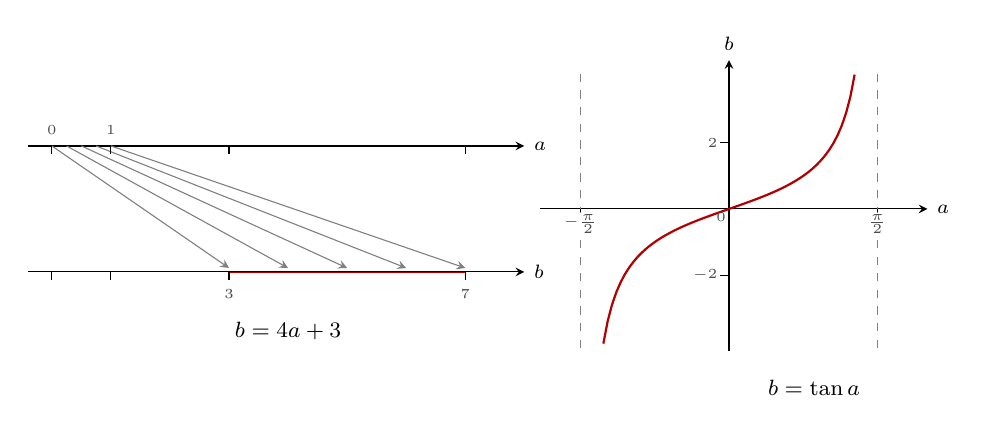
\begin{tikzpicture}
  \begin{scope}[x=0.75cm,y=1cm]
    \draw[thick,blue!60!black] (0,1.6) -- (1,1.6);
    \draw[->] (-0.4,1.6) -- (8,1.6) node[right,font=\scriptsize] {$a$};
    \draw[thick,red!70!black] (3,0) -- (7,0);
    \draw[->] (-0.4,0) -- (8,0) node[right,font=\scriptsize] {$b$};
    \foreach \a in {0,0.25,0.5,0.75,1}{\draw[gray,->] (\a,1.6) -- ({4*\a+3},0.05);}
    \foreach \p in {0,1,3,7}{\draw (\p,1.6) -- (\p,1.5); \draw (\p,0) -- (\p,-0.1);}
    \foreach \p in {0,1}{\node[font=\tiny,anchor=south,gray!60!black] at (\p,1.62) {$\p$};}
    \foreach \p in {3,7}{\node[font=\tiny,anchor=north,gray!60!black] at (\p,-0.1) {$\p$};}
    \node[font=\footnotesize] at (4,-0.75) {$b=4a+3$};
  \end{scope}
  \begin{scope}[shift={(8.6,0.8)},x=1.2cm,y=0.42cm]
    \draw[->] (-2,0) -- (2.1,0) node[right,font=\scriptsize] {$a$};
    \draw[->] (0,-4.3) -- (0,4.5) node[above,font=\scriptsize] {$b$};
    \draw[dashed,gray] (-1.5708,-4.2) -- (-1.5708,4.2);
    \draw[dashed,gray] (1.5708,-4.2) -- (1.5708,4.2);
    \draw[res,domain=-1.33:1.33,samples=60] plot (\x,{tan(deg(\x))});
    \xt{-1.5708}{-\frac{\pi}{2}}\xt{1.5708}{\frac{\pi}{2}}
    \yt{2}{2}\yt{-2}{-2}
    \node[anchor=north east,font=\tiny,gray!60!black,inner sep=1pt] at (0,-0.02) {$0$};
    \node[font=\footnotesize] at (0.9,-5.4) {$b=\tan a$};
  \end{scope}
\end{tikzpicture}
\caption{左：$[0,1]$ 上每个点线性对应到 $[3,7]$ 上一个点。右：$\tan a$ 把 $\left(-\frac\pi2,\frac\pi2\right)$ 一一对应到整条实数轴。}
\end{figure}

\example{线段与正方形一样多}{交错取位}{}
\textbf{题目}：线段 $[0,1]$ 上的点，与单位正方形 $[0,1]\times[0,1]$ 上的点，哪个多？

\textbf{解}：一样多。正方形上的点写成 $(a,b)$，$a,b\in[0,1]$；把 $a$、$b$ 的小数位\textbf{交错}抄成一个数 $c$：
\[
a=0.7182\cdots,\quad b=0.5436\cdots
\quad\Longrightarrow\quad
c=0.7\,5\,1\,4\,8\,3\,2\,6\cdots
\]
（$c$ 的奇数位来自 $a$，偶数位来自 $b$。）反过来，从 $c$ 的奇数位、偶数位又能拆回 $a$ 和 $b$。这建立了正方形与线段之间的一一对应。

\begin{note}
严格的证明还要处理 $0.0999\cdots=0.1$ 这类有两种小数写法的数，这里只讲构造思路。
\end{note}

%==================================================================
\section{性质三：与冲激相乘}\label{sec:p3}
\begin{remember}
\[
x(t)\,\delta(t)=x(0)\,\delta(t)\qquad(\text{教材第 12 页式 1-42}).
\]
变形：
\[
x(t)\,\delta(t-t_0)=x(t_0)\,\delta(t-t_0).
\]
这里的「$=$」按定义三理解。
\end{remember}

\point{证明（基于定义三）。}对任意 $y(t)$，比较两边与 $y(t)$ 相乘后的积分：
\begin{align*}
\text{左边：}\int_{-\infty}^{+\infty}y(t)\big[x(t)\,\delta(t)\big]\mathrm{d}t
&=\int_{-\infty}^{+\infty}\big[x(t)\,y(t)\big]\delta(t)\,\mathrm{d}t=x(0)\,y(0),\\
\text{右边：}\int_{-\infty}^{+\infty}y(t)\big[x(0)\,\delta(t)\big]\mathrm{d}t
&=x(0)\int_{-\infty}^{+\infty}y(t)\,\delta(t)\,\mathrm{d}t=x(0)\,y(0).
\end{align*}
左边把 $x(t)y(t)$ 整体看成一个函数，用性质二；右边先把常数 $x(0)$ 提出来，再用性质二。两边相等，由定义三，命题成立。变形的证明完全一样：两边乘 $y(t)$ 再积分，用性质二的变形。

\begin{figure}[H]
\centering
\begin{tikzpicture}[x=1.1cm,y=1.0cm]
  \begin{scope}
    \taxes{-2}{2.6}{2.6}
    \draw[thick,gray!60!black,dashed,domain=-1.8:2.3,samples=60] plot (\x,{1.5+0.4*sin(70*\x)});
    \imp{0}{1.9}{$(1)$}
    \xt{-1}{-1}\xt{1}{1}\xt{2}{2}\yt{1.5}{x(0)}
    \node[anchor=west,font=\footnotesize] at (1.2,2.15) {$x(t)$ 与 $\delta(t)$};
  \end{scope}
  \draw[->,thick] (3.2,1.2) -- (4.4,1.2) node[midway,above,font=\scriptsize] {相乘};
  \begin{scope}[shift={(6.6,0)}]
    \taxes{-2}{2.6}{2.6}
    \imp{0}{1.9}{$(x(0))$}
    \xt{-1}{-1}\xt{1}{1}\xt{2}{2}
    \node[anchor=west,font=\footnotesize] at (0.6,1.4) {$x(0)\,\delta(t)$};
  \end{scope}
\end{tikzpicture}
\caption{$x(t)$ 乘冲激，只有 $t=0$ 处的值 $x(0)$ 起作用：结果是强度为 $x(0)$ 的冲激（括号里的数是强度，不是高度）。}
\end{figure}

%==================================================================
\section{性质四：尺度变换}\label{sec:p4}
\begin{remember}
\[
\delta(at)=\frac{1}{|a|}\,\delta(t),\quad a\ne0\qquad(\text{教材第 24 页式 1-82}).
\]
变形：
\[
\delta(at+b)=\frac{1}{|a|}\,\delta\!\left(t+\frac ba\right).
\]
\end{remember}

\point{证明（基于定义三）。}对任意 $y(t)$：

右边：$\displaystyle\int_{-\infty}^{+\infty}y(t)\,\frac1{|a|}\,\delta(t)\,\mathrm{d}t=\frac1{|a|}\,y(0)$（性质二）。

左边：$\displaystyle\int_{-\infty}^{+\infty}y(t)\,\delta(at)\,\mathrm{d}t$，换元 $t'=at$，$t=\frac{t'}a$，$\mathrm{d}t=\frac{\mathrm{d}t'}a$。要按 $a$ 的正负讨论积分上下限：
\begin{enumerate}[nosep]
\item $a>0$：$t$ 从 $-\infty$ 到 $+\infty$ 时，$t'$ 也从 $-\infty$ 到 $+\infty$，
\[
\text{左边}=\frac1a\int_{-\infty}^{+\infty}y\!\left(\frac{t'}a\right)\delta(t')\,\mathrm{d}t'=\frac1a\,y(0).
\]
\item $a<0$：$t$ 从 $-\infty$ 到 $+\infty$ 时，$t'$ 从 $+\infty$ 到 $-\infty$，上下限颠倒，翻回来要加负号，
\[
\text{左边}=\frac1a\int_{+\infty}^{-\infty}y\!\left(\frac{t'}a\right)\delta(t')\,\mathrm{d}t'
=-\frac1a\int_{-\infty}^{+\infty}y\!\left(\frac{t'}a\right)\delta(t')\,\mathrm{d}t'=-\frac1a\,y(0).
\]
\end{enumerate}
两种情况合起来，左边 $=\frac1{|a|}y(0)=$ 右边。由定义三，命题成立。变形用同样的方法证明。

\begin{figure}[H]
\centering
\begin{tikzpicture}[x=2.2cm,y=1.0cm]
  \begin{scope}
    \taxes{-0.4}{1.5}{2.2}
    \fill[blue!12] (0,0) rectangle (0.8,1.6);
    \draw[sig] (0,0) -- (0,1.6) -- (0.8,1.6) -- (0.8,0);
    \xt{0.8}{\Delta}\yt{1.6}{\frac{1}{\Delta}}
    \node[anchor=west,font=\footnotesize] at (0.05,2.0) {$\delta_\Delta(t)$：面积 $1$};
  \end{scope}
  \begin{scope}[shift={(2.6,0)}]
    \taxes{-0.4}{1.5}{2.2}
    \fill[blue!12] (0,0) rectangle (0.4,1.6);
    \draw[sig] (0,0) -- (0,1.6) -- (0.4,1.6) -- (0.4,0);
    \draw[dashed,gray] (0.4,1.6) -- (0.8,1.6) -- (0.8,0);
    \xt{0.4}{\frac{\Delta}{2}}\xt{0.8}{\Delta}\yt{1.6}{\frac{1}{\Delta}}
    \node[anchor=west,font=\footnotesize] at (0.05,2.0) {$\delta_\Delta(2t)$：面积 $\frac12$};
  \end{scope}
\end{tikzpicture}
\caption{以 $a=2$ 为例：$\delta_\Delta(2t)$ 宽度压缩一半、高度不变，面积变成 $\frac12$。取极限得 $\delta(2t)=\frac12\delta(t)$。}
\end{figure}

%==================================================================
\section{函数相等与卷积}\label{sec:conv}
定义三下的「相等」和卷积完全兼容，可以放心地用来分析 LTI 系统。

\begin{remember}
\textbf{定理}：若 $h_1(t)=h_2(t)$（按定义三），则对任意 $x(t)$，有
\[
x(t)\ast h_1(t)=x(t)\ast h_2(t).
\]
逆命题也成立：若对任意 $x(t)$ 都有 $x(t)\ast h_1(t)=x(t)\ast h_2(t)$，则 $h_1(t)=h_2(t)$。
\end{remember}

\point{为什么需要证明。}按定义三，$h_1=h_2$ 并不保证两者每一点都相等，所以「代进卷积公式结果一样」不是显然的。

\point{证明。}
\begin{align*}
x(t)\ast h_1(t)
&=\int_{-\infty}^{+\infty}x(\tau)\,h_1(t-\tau)\,\mathrm{d}\tau
&&\text{（连续卷积公式）}\\
&=\int_{-\infty}^{+\infty}x(t-\tau)\,h_1(\tau)\,\mathrm{d}\tau
&&\text{（换元，即卷积交换律）}\\
&=\int_{-\infty}^{+\infty}x(t-\tau)\,h_2(\tau)\,\mathrm{d}\tau
&&\text{（定义三，把 $x(t-\tau)$ 当作 $y(\tau)$）}\\
&=x(t)\ast h_2(t).
\end{align*}

\point{第二个等号的换元。}令 $\tau'=t-\tau$，则 $\tau=t-\tau'$，$\mathrm{d}\tau=-\mathrm{d}\tau'$；$\tau=-\infty$ 时 $\tau'=+\infty$，$\tau=+\infty$ 时 $\tau'=-\infty$。于是
\[
\int_{-\infty}^{+\infty}x(\tau)\,h_1(t-\tau)\,\mathrm{d}\tau
=\int_{+\infty}^{-\infty}x(t-\tau')\,h_1(\tau')\,(-\mathrm{d}\tau')
=\int_{-\infty}^{+\infty}x(t-\tau')\,h_1(\tau')\,\mathrm{d}\tau',
\]
最后把 $\tau'$ 改写回 $\tau$ 即可。

\point{第三个等号。}对固定的 $t$，$x(t-\tau)$ 是 $\tau$ 的一个函数，相当于定义三中的 $y(\tau)$；$h_1=h_2$ 意味着它与 $h_1(\tau)$、$h_2(\tau)$ 分别相乘积分的结果相同。

%==================================================================
\section{性质五：冲激的复合}\label{sec:p5}
\begin{remember}
设 $f(t)$ 的所有零点为 $t_i$（即 $f(t_i)=0$），且 $f'(t_i)\ne0$，则
\[
\delta\big(f(t)\big)=\sum_{i}\frac{1}{|f'(t_i)|}\,\delta(t-t_i).
\]
这条性质出自郑君里《信号与系统》；证明方法仍是两边乘 $y(t)$ 再积分。
\end{remember}

$f(t)$ 每过一次零点，$\delta(f(t))$ 就在那里产生一个冲激，强度是该点斜率绝对值的倒数：$f(t)$ 穿过零点越陡，冲激越弱。

\example{性质四是性质五的特例}{\texorpdfstring{$f(t)=at$}{f(t)=at}}{}
取 $f(t)=at$（$a\ne0$）。当且仅当 $t=0$ 时 $f(t)=0$；$f'(t)=a$，所以 $f'(0)=a$。代入性质五：
\[
\delta(at)=\frac1{|a|}\,\delta(t),
\]
正是性质四。

\example{\texorpdfstring{$\delta(t^2-3t+2)$}{δ(t²-3t+2)}}{\texorpdfstring{$\delta(t-1)+\delta(t-2)$}{δ(t-1)+δ(t-2)}}{}
\textbf{解}：$f(t)=t^2-3t+2=(t-1)(t-2)$，当且仅当 $t=1$、$t=2$ 时 $f(t)=0$。$f'(t)=2t-3$，所以 $f'(1)=-1$，$f'(2)=1$。代入性质五：
\[
\delta(t^2-3t+2)=\frac1{|-1|}\,\delta(t-1)+\frac1{|1|}\,\delta(t-2)=\delta(t-1)+\delta(t-2).
\]

\begin{figure}[H]
\centering
\begin{tikzpicture}[x=1.2cm,y=0.9cm]
  \begin{scope}
    \taxes{-0.5}{3.4}{2.4}
    \draw[res,domain=0:3.1,samples=60] plot (\x,{\x*\x-3*\x+2});
    \draw[dashed,gray] (1,0) -- (1.6,-0.6);
    \draw[dashed,gray] (2,0) -- (2.6,0.6);
    \foreach \p in {1,2,3}{\xt{\p}{\p}}\yt{1}{1}\yt{2}{2}
    \node[anchor=west,font=\scriptsize] at (1.6,-0.7) {斜率 $-1$};
    \node[anchor=west,font=\scriptsize] at (2.6,0.6) {斜率 $1$};
    \node[anchor=west,font=\footnotesize] at (0.15,2.25) {$f(t)=t^2-3t+2$};
  \end{scope}
  \begin{scope}[shift={(6.0,0)}]
    \taxes{-0.5}{3.4}{2.4}
    \imp{1}{1.5}{$(1)$}\imp{2}{1.5}{$(1)$}
    \foreach \p in {1,2,3}{\xt{\p}{\p}}
    \node[anchor=west,font=\footnotesize] at (0.15,2.25) {$\delta\big(f(t)\big)$};
  \end{scope}
\end{tikzpicture}
\caption{左：$f(t)$ 在 $t=1$、$t=2$ 处过零，斜率分别为 $-1$、$1$。右：$\delta(f(t))$ 在这两点各有一个强度为 $1$ 的冲激。}
\end{figure}

\example{\texorpdfstring{$\delta(\cos t)$ 与 $\delta(\sin t)$}{δ(cos t) 与 δ(sin t)}}{\texorpdfstring{每隔 $\pi$ 一个冲激}{每隔 π 一个冲激}}{}
\textbf{解}：设 $f(t)=\cos t$，当且仅当 $t=k\pi+\frac\pi2$（$k\in\mathbb{Z}$）时 $f(t)=0$。$f'(t)=-\sin t$，
\[
\left|f'\!\left(k\pi+\tfrac\pi2\right)\right|=\left|\sin\!\left(k\pi+\tfrac\pi2\right)\right|=1
\]
（正负交替，但绝对值恒为 $1$）。代入性质五：
\[
\delta(\cos t)=\sum_{k=-\infty}^{+\infty}\delta\!\left(t-k\pi-\frac\pi2\right).
\]
同理，$\sin t$ 的零点是 $t=k\pi$，且 $|\cos k\pi|=1$，所以
\[
\delta(\sin t)=\sum_{k=-\infty}^{+\infty}\delta(t-k\pi).
\]

\example{\texorpdfstring{$\int_{-2\pi}^{2\pi}(1+t)\,\delta(\cos t)\,\mathrm{d}t$}{含 δ(cos t) 的积分}}{结果为 4}{教材第 33 页 1-20(3)}
\textbf{解}：由上一例，$\delta(\cos t)$ 在每个 $k\pi+\frac\pi2$ 处有一个强度为 $1$ 的冲激。积分区间 $[-2\pi,2\pi]$ 里只有四个：$-\frac{3\pi}2,\ -\frac\pi2,\ \frac\pi2,\ \frac{3\pi}2$（$\pm\frac{5\pi}2$ 在区间外）。

\begin{figure}[H]
\centering
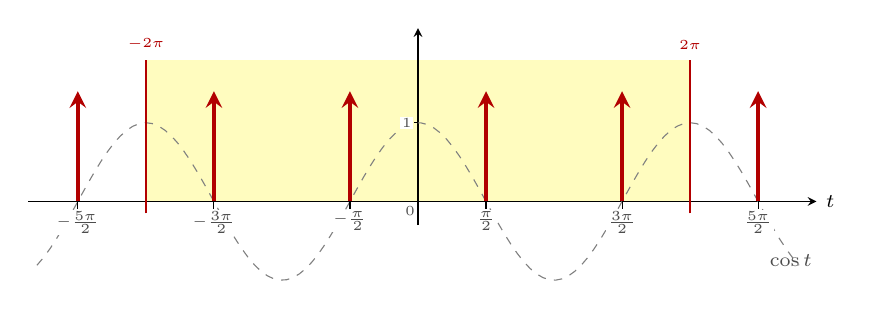
\begin{tikzpicture}[x=0.55cm,y=1.0cm]
  \fill[yellow!25] (-6.2832,0) rectangle (6.2832,1.8);
  \taxes{-9}{9.2}{2.2}
  \draw[gray,dashed,domain=-8.8:8.8,samples=120] plot (\x,{cos(deg(\x))});
  \foreach \k in {-7.854,-4.712,-1.5708,1.5708,4.712,7.854}{\imp{\k}{1.4}{}}
  \draw[red!70!black,thick] (-6.2832,-0.15) -- (-6.2832,1.8);
  \draw[red!70!black,thick] (6.2832,-0.15) -- (6.2832,1.8);
  \node[font=\tiny,red!70!black,anchor=south] at (-6.2832,1.8) {$-2\pi$};
  \node[font=\tiny,red!70!black,anchor=south] at (6.2832,1.8) {$2\pi$};
  \xt{-7.854}{-\frac{5\pi}{2}}\xt{-4.712}{-\frac{3\pi}{2}}\xt{-1.5708}{-\frac{\pi}{2}}
  \xt{1.5708}{\frac{\pi}{2}}\xt{4.712}{\frac{3\pi}{2}}\xt{7.854}{\frac{5\pi}{2}}
  \yt{1}{1}
  \node[anchor=west,font=\scriptsize,gray!60!black] at (7.9,-0.75) {$\cos t$};
\end{tikzpicture}
\caption{灰色虚线是 $\cos t$，红色箭头是 $\delta(\cos t)$ 的冲激（强度均为 $1$），落在 $\cos t$ 的每个零点上。黄色是积分区间 $[-2\pi,2\pi]$，里面只有四个冲激。}
\end{figure}

\[
\int_{-2\pi}^{2\pi}(1+t)\,\delta(\cos t)\,\mathrm{d}t
=\int_{-2\pi}^{2\pi}(1+t)\Big[\delta\!\left(t+\tfrac{3\pi}2\right)+\delta\!\left(t+\tfrac\pi2\right)+\delta\!\left(t-\tfrac\pi2\right)+\delta\!\left(t-\tfrac{3\pi}2\right)\Big]\mathrm{d}t .
\]
每一项用性质二的变形 $\int x(t)\,\delta(t-t_0)\,\mathrm{d}t=x(t_0)$（冲激在积分区间内部，积分限不必是 $\pm\infty$）：
\[
=\left(1-\tfrac{3\pi}2\right)+\left(1-\tfrac\pi2\right)+\left(1+\tfrac\pi2\right)+\left(1+\tfrac{3\pi}2\right)=4 .
\]
含 $\pi$ 的项两两抵消。

%==================================================================
\section{冲激函数的多样性}\label{sec:many}
\subsection{\texorpdfstring{判定一个函数是不是 $\delta(t)$}{判定一个函数是不是 δ(t)}}
$\delta(t)$ 不只有「$[0,\Delta]$ 上的窄方波取极限」这一种写法，很多不同的极限都等于它。判定方法：

\begin{remember}
要证明一个函数 $f(t)$ 是 $\delta(t)$，只需证明对任意函数 $y(t)$ 有
\[
\int_{-\infty}^{+\infty}y(t)\,f(t)\,\mathrm{d}t=y(0).
\]
\end{remember}
理由有两条：一是性质二，$\int y(t)\,\delta(t)\,\mathrm{d}t=y(0)$；二是定义三，与任意 $y(t)$ 相乘积分结果都相同的两个函数相等。

\subsection{对称的窄方波}
有的教材把 $\delta_\Delta(t)$ 定义为 $\left[-\frac\Delta2,\frac\Delta2\right]$ 上高度为 $\frac1\Delta$ 的方波，再令 $\Delta\to0$。两种定义都对。

\point{证明。}
\begin{align*}
\int_{-\infty}^{+\infty}y(t)\Big[\lim_{\Delta\to0}\delta_\Delta(t)\Big]\mathrm{d}t
&=\lim_{\Delta\to0}\frac1\Delta\int_{-\Delta/2}^{\Delta/2}y(t)\,\mathrm{d}t\\
&=\lim_{\Delta\to0}\frac1\Delta\cdot y(\xi)\,\Delta,\quad -\tfrac\Delta2\le\xi\le\tfrac\Delta2
&&\text{（积分中值定理）}\\
&=\lim_{\Delta\to0}y(\xi)=y(0).
\end{align*}

\subsection{三角形脉冲}
$\delta_\Delta(t)$ 取底边为 $[-\Delta,\Delta]$、顶点高度为 $\frac1\Delta$ 的三角形（面积 $\frac12\cdot2\Delta\cdot\frac1\Delta=1$），$\Delta\to0$ 时同样等于 $\delta(t)$。证明方法相同，只是积分要分左右两段讨论，计算更繁琐。

\begin{figure}[H]
\centering
\begin{tikzpicture}[x=1.6cm,y=1.0cm]
  \begin{scope}
    \taxes{-1.1}{1.3}{2.3}
    \fill[blue!12] (0,0) rectangle (0.6,1.7);
    \draw[sig] (0,0) -- (0,1.7) -- (0.6,1.7) -- (0.6,0);
    \xt{0.6}{\Delta}\yt{1.7}{\frac{1}{\Delta}}
    \node[font=\footnotesize] at (0.1,-0.8) {$[0,\Delta]$ 方波};
  \end{scope}
  \begin{scope}[shift={(3.0,0)}]
    \taxesn{-1.1}{1.3}{2.3}
    \fill[blue!12] (-0.3,0) rectangle (0.3,1.7);
    \draw[sig] (-0.3,0) -- (-0.3,1.7) -- (0.3,1.7) -- (0.3,0);
    \xt{-0.3}{-\frac{\Delta}{2}}\xt{0.3}{\frac{\Delta}{2}}
    \draw (0,1.7) -- (-0.1,1.7);
    \node[anchor=east,font=\tiny,gray!60!black,fill=white,inner sep=0.6pt] at (-0.32,1.7) {$\frac{1}{\Delta}$};
    \node[font=\footnotesize] at (0.1,-0.8) {对称方波};
  \end{scope}
  \begin{scope}[shift={(6.0,0)}]
    \taxesn{-1.1}{1.3}{2.3}
    \fill[blue!12] (-0.6,0) -- (0,1.7) -- (0.6,0) -- cycle;
    \draw[sig] (-0.6,0) -- (0,1.7) -- (0.6,0);
    \xt{-0.6}{-\Delta}\xt{0.6}{\Delta}\yt{1.7}{\frac{1}{\Delta}}
    \node[font=\footnotesize] at (0.1,-0.8) {三角形脉冲};
  \end{scope}
\end{tikzpicture}
\caption{三种 $\delta_\Delta(t)$，面积都是 $1$。$\Delta\to0$ 时三者都等于 $\delta(t)$。}
\end{figure}

\subsection{抽样函数的极限}\label{sec:sa}
\begin{remember}
\[
\lim_{\omega\to+\infty}\frac{\sin(\omega t)}{\pi t}=\delta(t).
\]
这个结论在第三章还会用到，即使记不住证明，也要\textbf{记住结论}。
\end{remember}

\point{直观理解。}$\dfrac{\sin(\omega t)}{\pi t}$ 是一个抽样函数（Sa 函数）的形状（$\omega>0$）：
\begin{itemize}[nosep]
\item $t=0$ 处取极限值 $\dfrac\omega\pi$；
\item 零点在 $t=\pm\dfrac\pi\omega,\ \pm\dfrac{2\pi}\omega,\dots$；
\item $\displaystyle\int_{-\infty}^{+\infty}\frac{\sin(\omega t)}{\pi t}\,\mathrm{d}t=1$，与 $\omega$ 无关。
\end{itemize}
$\omega\to+\infty$ 时，中间的峰冲向无穷大，零点 $\frac\pi\omega\to0$，整个波浪被向中间无限压缩、两侧被压平；而面积始终为 $1$，和性质一吻合。看起来就像一个冲激。

\begin{figure}[H]
\centering
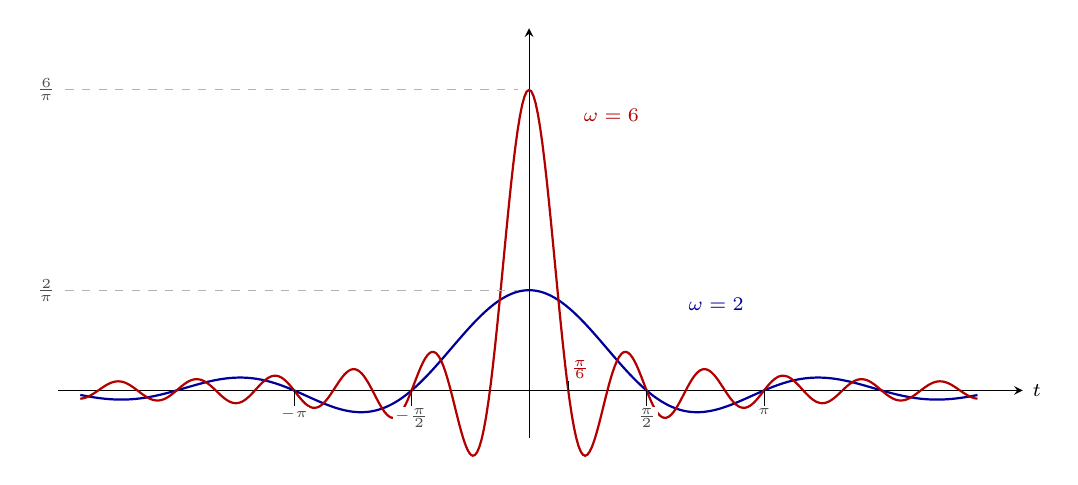
\begin{tikzpicture}[x=0.95cm,y=2.0cm]
  \taxesn{-6.3}{6.6}{2.3}
  \draw[thick,blue!60!black,domain=-6:6,samples=399] plot (\x,{sin(deg(2*\x))/(pi*\x)});
  \draw[thick,red!70!black,domain=-6:6,samples=399] plot (\x,{sin(deg(6*\x))/(pi*\x)});
  \xt{1.5708}{\frac{\pi}{2}}\xt{-1.5708}{-\frac{\pi}{2}}\xt{3.1416}{\pi}\xt{-3.1416}{-\pi}
  \draw (0.5236,0) -- (0.5236,0.06) node[anchor=south west,font=\tiny,red!70!black,fill=white,inner sep=0.6pt] {$\frac{\pi}{6}$};
  \foreach \v/\l in {0.6366/\frac{2}{\pi},1.9099/\frac{6}{\pi}}{%
    \draw[dashed,gray!60] (-6.2,\v) -- (-0.15,\v);
    \node[anchor=east,font=\tiny,gray!60!black] at (-6.2,\v) {$\l$};}
  \node[anchor=west,font=\scriptsize,blue!60!black] at (2.0,0.55) {$\omega=2$};
  \node[anchor=west,font=\scriptsize,red!70!black] at (0.6,1.75) {$\omega=6$};
\end{tikzpicture}
\caption{$\frac{\sin(\omega t)}{\pi t}$。蓝：$\omega=2$，峰值 $\frac2\pi$，第一个零点 $\frac\pi2$；红：$\omega=6$，峰值 $\frac6\pi$，第一个零点 $\frac\pi6$。两条水平虚线标出两个峰值。$\omega$ 越大，峰越高越窄，面积始终为 $1$。}
\end{figure}

\point{引理。}若 $x(t)$ 不是无限振荡的函数，则
\[
\lim_{\omega\to+\infty}\int_{-\infty}^{+\infty}x(t)\cos(\omega t)\,\mathrm{d}t=0,\qquad
\lim_{\omega\to+\infty}\int_{-\infty}^{+\infty}x(t)\sin(\omega t)\,\mathrm{d}t=0 .
\]
\textbf{直观理解}：$\omega$ 很大时 $\cos(\omega t)$ 上下振荡极快。相邻的半个周期里，$\cos$ 一正一负，而 $x(t)$ 变化平缓、取值几乎一样，所以 $x(t)\cos(\omega t)$ 在相邻两段上的积分一正一负、互相抵消，总积分趋于 $0$。只有 $x(t)$ 自己也变化得极其剧烈（无限振荡），才抵消不掉。

\begin{figure}[H]
\centering
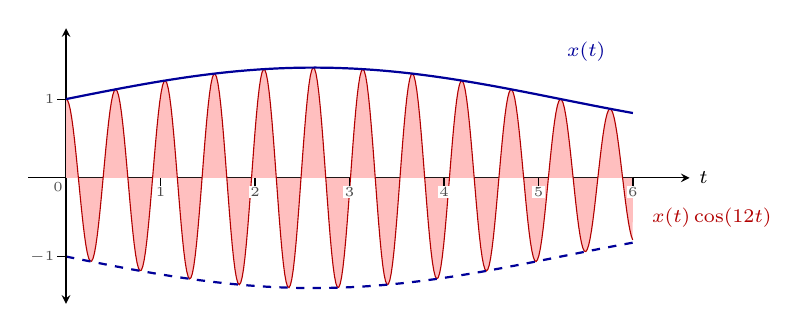
\begin{tikzpicture}[x=1.2cm,y=1.0cm]
  \taxes{-0.4}{6.6}{1.9}
  \draw[draw=none,fill=red!25,domain=0:6,samples=400] plot (\x,{(1+0.4*sin(deg(0.6*\x)))*cos(deg(12*\x))}) -- (6,0) -- (0,0) -- cycle;
  \draw[red!70!black,domain=0:6,samples=400] plot (\x,{(1+0.4*sin(deg(0.6*\x)))*cos(deg(12*\x))});
  \draw[thick,blue!60!black,domain=0:6,samples=60] plot (\x,{1+0.4*sin(deg(0.6*\x))});
  \draw[thick,blue!60!black,dashed,domain=0:6,samples=60] plot (\x,{-(1+0.4*sin(deg(0.6*\x)))});
  \foreach \p in {1,...,6}{\xt{\p}{\p}}
  \yt{1}{1}
  \draw (0,-1) -- (-0.1,-1) node[anchor=east,font=\tiny,gray!60!black,fill=white,inner sep=0.6pt] {$-1$};
  \draw[->] (0,-0.3) -- (0,-1.6);
  \node[anchor=west,font=\scriptsize,blue!60!black] at (5.2,1.6) {$x(t)$};
  \node[anchor=west,font=\scriptsize,red!70!black] at (6.1,-0.5) {$x(t)\cos(12t)$};
\end{tikzpicture}
\caption{蓝线是平缓的 $x(t)$，红色是 $x(t)\cos(\omega t)$（$\omega=12$）。正、负两部分面积几乎一样，积分几乎为 $0$；$\omega$ 越大抵消越彻底。}
\end{figure}

\point{引理在 $x(t)$ 可导时的证明。}用分部积分：
\begin{align*}
\int_{-\infty}^{+\infty}x(t)\cos(\omega t)\,\mathrm{d}t
&=\frac1\omega\int_{-\infty}^{+\infty}x(t)\,\mathrm{d}\big(\sin(\omega t)\big)\\
&=\frac1\omega\Big[x(t)\sin(\omega t)\Big]_{-\infty}^{+\infty}-\frac1\omega\int_{-\infty}^{+\infty}x'(t)\sin(\omega t)\,\mathrm{d}t .
\end{align*}
方括号和后面的积分都是有限值，前面乘 $\frac1\omega$；$\omega\to+\infty$ 时两项都趋于 $0$。$\sin$ 的情况同理。（只要求 $x(t)$ 不是无限振荡的版本更一般，证明更难。）

\point{证明 $\lim\limits_{\omega\to+\infty}\frac{\sin(\omega t)}{\pi t}=\delta(t)$。}由判定方法，只需证明对任意 $y(t)$：
\[
\int_{-\infty}^{+\infty}\Big[\lim_{\omega\to+\infty}\frac{\sin(\omega t)}{\pi t}\Big]y(t)\,\mathrm{d}t=y(0).
\]
左边 $=\lim\limits_{\omega\to+\infty}\displaystyle\int_{-\infty}^{+\infty}\frac{y(t)}{\pi t}\sin(\omega t)\,\mathrm{d}t$。

\textbf{不能直接套引理}：若 $y(0)\ne0$，$\frac{y(t)}{\pi t}$ 在 $t\to0^-$ 时趋于 $\mp\infty$、$t\to0^+$ 时趋于 $\pm\infty$，在 $0$ 点附近变化无限剧烈，不满足引理的条件。

\textbf{做法}：减一个 $y(0)$ 再加回来：
\[
\text{左边}=\underbrace{\lim_{\omega\to+\infty}\int_{-\infty}^{+\infty}\frac{y(t)-y(0)}{\pi t}\sin(\omega t)\,\mathrm{d}t}_{(\text{A})}
+\;y(0)\underbrace{\lim_{\omega\to+\infty}\int_{-\infty}^{+\infty}\frac{\sin(\omega t)}{\pi t}\,\mathrm{d}t}_{(\text{B})}.
\]
\begin{itemize}[nosep]
\item (A)：设 $x(t)=\dfrac{y(t)-y(0)}{\pi t}$。$t\to0$ 时分子、分母都趋于 $0$，由洛必达法则 $x(0)=\lim\limits_{t\to0}\dfrac{y'(t)}{\pi}=\dfrac{y'(0)}{\pi}$，即
\[
x(t)=\begin{cases}\dfrac{y(t)-y(0)}{\pi t},&t\ne0\\[6pt]\dfrac{y'(0)}{\pi},&t=0\end{cases},
\]
不再是无限振荡的函数，可以用引理：(A) $=0$。
\item (B)：对任意 $\omega>0$，积分恒等于 $1$，所以 (B) $=1$。
\end{itemize}
因此左边 $=0+y(0)\cdot1=y(0)$，命题成立。

\subsection{另一个例子}
\[
\lim_{\tau\to0}\frac{\tau}{\pi\,(t^2+\tau^2)}=\delta(t)
\]
也成立（郑君里《信号与系统》习题集）。

\end{document}
